\chapter{Interaction with the Environment and Model Identification Methods}
\label{chapter: interaction_with_env_and_model_identification}
\textit{This chapter will provide an overview of \textbf{model identification methods} and \textbf{controllers} for robot interaction with the environment. Interaction includes for example robot driving, or push manipulation. A system model estimates the true dynamics of one, or multiple objects. A system model can be learned with system identification methods. Different model representations are categorised in \cref{section: system_model_representation}. In this report, the controllers' focus is on tracking a reference signal. Not all, but the majority of controllers require a system model to determine system input. The controllers are categorised in \cref{section: interaction_approaches_and_model_iden_methods}. For models and controllers, a distinction is made for one body (e.g. the robot itself) and for multiple bodies (e.g. the robot pushing a ball). Performance and limitations are discussed in \cref{section: controllers_discussion}.
}

\section{System Model Representation}
\label{section: system_model_representation}
Let's first clarify the use of system models. The goal of system models is to capture the true dynamics of the system it describes. For instance, consider the following examples: when a robot arm reaches for some product to pick, a system model can estimate how the robot arm reacts before actually sending the input. Or consider a sphere which has received a push, the behaviour after the push is different from a cube which received an equal push, thus their models must be different also. A system model combined with the current state of the system and potential system input can estimate the state a system will be in as a result of the system input. An example of system input is wheel velocity $\omega_l$ and $\omega_r$ in \cref{fig: 2D_representation_robot}. State information and the effect of system input are crucial information for robot control design, and for controllers to operate effectively, robot controllers will be discussed in the next section.\\

Models investigated in this literature are split into 2 other categories, single-body models and multi-body models. Such a distinction is made because both models have quite different dynamical properties, let's first define both. A \textbf{single-body model} is a system model which estimates the true dynamics of an object, which is assumed to be connected for all times. An example is a robot arm existing of multiple parts which are connected by joints (assuming that a part of the robot arm does not break off). The robot arm is a single-body and any model estimating only the true dynamics of only the robot arm belongs to the set of single-body models. \textbf{Multi-body models} are system models which estimate the true dynamics which involve multiple objects. These multiple objects can be connected or disconnected. Multi-body models include any combination of single-/multi- body models with other single-/multi-body models. For example, a robot arm grasping a box with a gripper. For the period the box is grasped by the robot gripper, the single-body model estimating the true dynamics of the robot arm can be augmented such that it estimates the pose of the box. Such an augmented model belongs to the set of multi-body models.\\

The true dynamics of a single-body contain some nonlinear parts such as slip and friction, however in general nonlinear dynamics are not dominating such that a single-body system can be estimated with \ac{LTI} models. Dynamics which allow simplification to a linear model dominate compared to the nonlinear dynamics of the true dynamics, small accumulating errors as a result of for example slip can be accounted for. Stable control using \ac{LTI} models is possible because the true dynamcis can be estimated by an \ac{LTI} system model. Opposed to single-body system, multi-body systems are dominated by nonlinear dynamics, so much that a simplification to a linear system erases most true dynamics. Such a compromise for multi-body models is undesired since it would lead to a model mismatch between the model and the true dynamics, motivating the separation of single- and multi-body models.

\subsection{Example Model}


\begin{figure}[ht]
\centering
\begin{subfigure}{.5\textwidth}
 \centering
    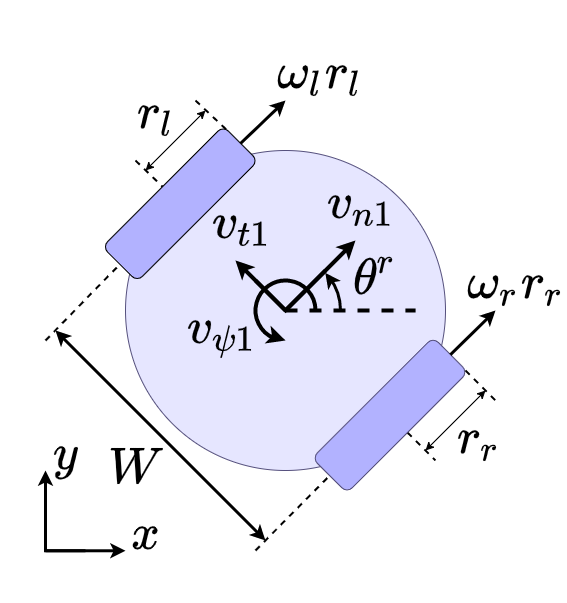
\includegraphics[width=0.8\textwidth]{figures/schematic_differential_drive_robot.png}
    \caption{Schematic 2D diagram of differential drive robot in world frame $<x, y, \theta>$, the robots frame's origin is located at $(x^r, y^r, \theta^r)$ and denoted as $<n1, t1, \psi1>$. The robot frames origin is where the robot's center of mass is located. The robot's left wheel has radius $r_l$, the right wheel has radius $r_r$, the robot wheels act upon the ground in the center of the wheel. The distance between where the left and right act upon the ground is notated as $W$. The angular speed of the left and right wheels are denoted by $\omega_l$ and $\omega_r$ respectively.}
    \label{fig: 2D_representation_robot}
\end{subfigure}%
\begin{subfigure}{.5\textwidth}
  \centering
 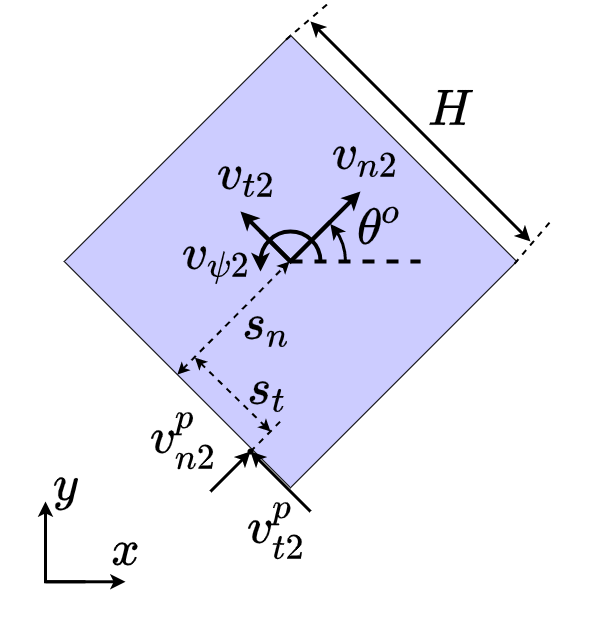
\includegraphics[width=0.8\textwidth]{figures/schematic_square_object.png}
    \caption{Schematic 2D diagram of cube object in world frame $<x, y, \theta>$, the object frame's origin is located at $(x^o, y^o, \theta^o)$ and denoted as $<n2, t2, \psi2>$. The object frames origin is where the cube's center of mass is located. Both length and width of the cube are $H$. A contact point $p$ is located at $s$ which can be decomposed in $s_n$ and $s_t$. An outside force pushes against at point $p$ the cube resulting in velocity component $v^p$ which can be decomposed in $v_{n2}^p$ and $v_{t2}^p$.}
    \label{fig: 2D_representation_object}
\end{subfigure}
\caption{Two example of single bodies}
\label{fig: single_body_models}
\end{figure}

let's consider an example system model, a differential drive mobile robot displayed in \cref{fig: 2D_representation_robot}. During design and construction, the robot can be fully analysed. When given the task to model the differential drive robot, it is thus reasonable to assume that some prior knowledge about the robot is known (e.g. weight or relation between forward velocity $v_{n1}$, wheel radiuses $r_l$, $r_r$, angular speeds $\omega_l$ and $\omega_r$). In that case, selecting and designing a \textit{differential equation} or \textit{parameterisable differential} equation is a logical option for reasons which will be discussed in  \cref{subsection: analytical_models,subsection: hybrid_models}. Literature reveals that a differential equation is a popular option to model a system \cite{bauza_data-efficient_2018, seegmiller_vehicle_2013}. Robots can come across a variety of objects, such as the cube object displayed in \cref{fig: 2D_representation_object}, both the differential drive robot and the cube object are modelled as differential equations displayed by \cref{equation: differential_equation_differential_robot} and \cref{equation: differential_equation_square_object} respectively.

\begin{equation}
\dot{\rho}^r(t)
=
\left[\begin{array}{l}
\dot{x}^r(t) \\
\dot{y}^r(t) \\
\dot{\theta}^r(t)
\end{array}\right]
=
f(\rho^r(t), u^r(t))
=
\left[\begin{array}{cc}
\cos (\theta^r(t)) & 0 \\
\sin (\theta^r(t)) & 0 \\
0 & 1
\end{array}\right]\left[\begin{array}{cc}
\frac{r_{l}}{2} & \frac{r_{r}}{2} \\
-\frac{r_{l}}{W} & \frac{r_{r}}{W}
\end{array}\right]\left[\begin{array}{l}
\omega_{l}(t) \\
\omega_{r}(t)
\end{array}\right]
\label{equation: differential_equation_differential_robot}
\end{equation}

\noindent With states $\rho^r(t) = \left[x^r(t) \quad y^r(t) \quad \theta^r(t)\right]^\top$, input $u^r(t)=\left[\omega_l(t) \quad \omega_r(t) \right]^\top$\\and constants $W$, $r_l$, $r_r$, $ > 0$. \Cref{equation: differential_equation_differential_robot}  from \cite{seegmiller_vehicle_2013}.\\

\Cref{equation: differential_equation_differential_robot} displays an analytical single-body model, if the equation would be expressed in robot frame it would be more compact because the transformation matrix (matrix containing both $\text{cos}(\theta^r(t))$ and $\text{sin}(\theta^r(t))$) is then scrapped, and instead of 3 state variables only two are sufficient. Later on, the two single bodies will be combined to one multi-body model, expressed in a world frame. For consistency, all system models accompanying the robot and cube example are in world frame.\\

\Cref{equation: differential_equation_square_object}  estimates the true dynamics of the cube object, because $v^p_{n2}$ acts upon the object, the object will translate and rotate. if the speed acts on the cube at the middle $s_t = 0$ then the speed will completely go to translation of the cube $v_{n2} = v^p_{n2}$. If the speeds acts on the cube at the corner $s_t = \pm \frac{H}{2}$, then the speed will completely go-to rotation of the cube, $\theta^o = v^p_{n2}s_t$. Linear interpolation between the middle and the corner points determines the ratio between translation and rotation, which is a function of speed $v^p_{n2}$  described as:

$$\dot{\theta}^o = \frac{2 s_t}{H} |s_t| v_{n2}^p$$
$$v_{n2} = (1-|\frac{2 s_t}{H}|) v_{n2}^p$$

yielding the following differential equation:

\begin{equation}
\dot{\rho}^o(t)
=
\left[\begin{array}{l}
\dot{x}^o(t) \\
\dot{y}^o(t) \\
\dot{\theta}^o(t)
\end{array}\right]
=
f(\rho^o(t), u^o(t))
=
\left[\begin{array}{c}
(1-|\frac{2 s_t}{H}|) \cos (\theta^o(t))v^p_{n2} \\
(1-|\frac{2 s_t}{H}|) \sin (\theta^o(t))v^p_{n2} \\
\frac{2 s_t}{H}|s_t|v^p_{n2}
\end{array}\right]
\label{equation: differential_equation_square_object}
\end{equation}

\noindent With states $\rho^o(t) = \left[x^o(t) \quad y^o(t) \quad \theta^o(t)\right]^\top$, input $u^o(t)=\left[v^p_{n2} \quad s_t\right]^\top $ \\and constant $H > 0$ and constraint $|s_t| \leq \frac{H}{2}$. \Cref{equation: differential_equation_square_object} is inspired by the analytical model in \cite{bauza_data-efficient_2018}.\\

\Cref{equation: differential_equation_square_object} is not approximating the true dynamics accurately, because pushing a cube using this differential equation does not capture any speed in the direction of the $t$-axis at point $p$. There is no friction of the object with the ground, let alone a distinction between static and dynamic friction which both affect the dynamics considerably. Simplifying the true dynamics results is model mismatch, too much simplification would eventually lead to a nonsense model, incapable of modelling the system behaviour accurately and leading to stability issues when used by a controller. \Cref{equation: differential_equation_square_object} simplifies too much and is thus an ineffective modelling method. However, for the purpose of an example \cref{equation: differential_equation_square_object} is sufficient. To improve modelling the true dynamics of a robot pushing a box, more details of the true dynamics should be captured. \cite{bauza_data-efficient_2018} created an analytical model for push manipulation involving Coulomb friction, force and friction constraints, resulting in a model modelled accurate enough to successfully track a reference signal. \cite{bauza_data-efficient_2018} performed a close inspection of the object to push. Assuming prior knowledge about the object to encounter is unrealistic as opposed to robot dynamics. Now the two single-body models will be combined as a multi-body model, a schematic 2D diagram is displayed in \cref{fig: multiple_body_diagram}. \\

\begin{figure}[H]
    \centering
    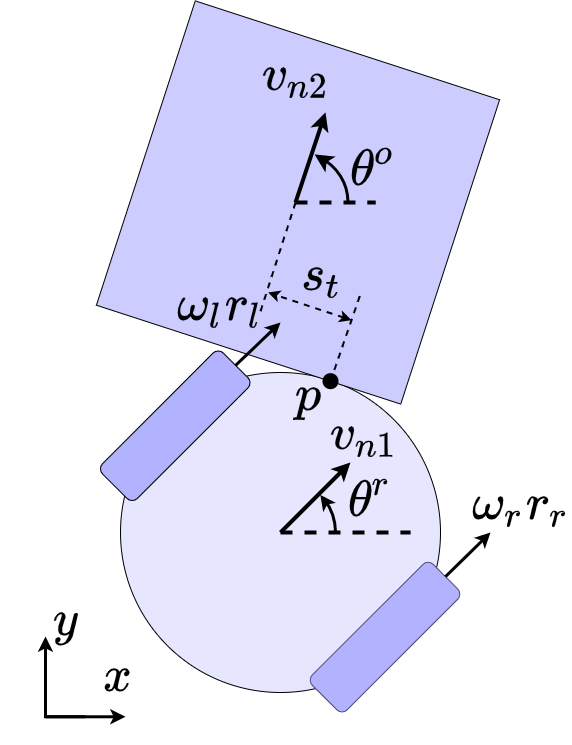
\includegraphics[width=0.38\textwidth]{figures/schematic_diff_drive_and_square.png}
    \caption{Combining single bodies \cref{fig: 2D_representation_robot,fig: 2D_representation_object} which are connected at contact point $p$ to create a multi body.}
    \label{fig: multiple_body_diagram}
\end{figure}

Augmenting the differential \cref{equation: differential_equation_differential_robot} with \cref{equation: differential_equation_square_object} creates a multi-body model:

\begin{equ}[H]
\begin{align}
\label{equation: multiple_body_model_robot_cube}
\dot{\rho}^{ro}(t)
&=
\left[\begin{array}{l}
\dot{x}^r(t) \\
\dot{y}^r(t) \\
\dot{\theta}^r(t) \\
\dot{x}^o(t) \\
\dot{y}^o(t) \\
\dot{\theta}^o(t)
\end{array}\right]
=
f(\rho^{ro}(t), u^r(t))\\ 
&=
\left[\begin{array}{ccc}
\cos(\theta^r(t)) & 0 & 0\\
\sin(\theta^r(t)) & 0 & 0\\
0 & 1 & 0 \\
0 & 0 & (1-|\frac{2 s_t}{H}|) \cos (\theta^o(t)) \\
0 & 0 & (1-|\frac{2 s_t}{H}|) \sin (\theta^o(t))\\
0 & 0 & \frac{2 s_t}{H}|s_t|
\end{array}\right]
\left[\begin{array}{cccc}
1& 0 \\
0 & 1 \\
cos(\theta^r(t) - \theta^o(t)) & 0 \\
\end{array}\right]
\left[\begin{array}{cc}
\frac{r_{l}}{2} & \frac{r_{r}}{2} \\
-\frac{r_{l}}{W} & \frac{r_{r}}{W}\\
\end{array}\right]
\left[\begin{array}{l}
\omega_{l}(t) \\
\omega_{r}(t) \\
\end{array}\right] \nonumber
\end{align}
\caption*{Combining both single-body models displayed in \cref{equation: differential_equation_differential_robot,equation: differential_equation_square_object} to obtain a multi-body model.}
\end{equ}

with $s_t$ now dependent on both the location and geometric properties of the robot and the object, defined as:

$$
s_t = \sqrt{(x^o(t)-x^r(t)-\frac{H+W}{2}cos(\theta^o(t)))^2 + (y^o(t)-y^r(t)-\frac{H+W}{2}sin(\theta^o(t))^2}
$$

The multi-body model in \cref{equation: multiple_body_model_robot_cube} displays how the first derivative of state variables can be calculated based on the input $u^r(t) = \left[\omega_l \quad \omega_r \right]$, the system constants $H$, $r_l$, $r_r$, $W$ and the state variables. The multi-body model estimates the true dynamics of the robot and the box. The robot and cube object are touching at point $p$, when the objects become disjoint the multi-object model is not a valid representation of the true dynamics any more. \\

This concludes the example of multiple single-body models into a multi-body model. In the example, we saw one way of analytically modelling a robot and an cube object. There is however a vast literature of different methods which could been applied to model \cref{fig: multiple_body_diagram} \cite{nascimento_nonholonomic_2018}, \cite{bauza_data-efficient_2018}, \cite{stuber_feature-based_2018}, \cite{stuber_lets_2020}. An overview of modelling methods reviewed is conveniently condensed into \cref{mindmap: classify_system_models}. Now the distinction between single-body models and multi-body models is clear, and the advantages and disadvantages per class of models are discussed.

\begin{figure}[h]
\centering
\resizebox{!}{11cm}{%
\begin{tikzpicture}[
    mindmap,
    concept color = myDarkColor,
    every node/.style = {concept},
    grow cyclic,
    level 1/.append style = {
        concept color = myLightColor,
        level distance = 4.4cm,
        sibling angle = 120
    },
    level 2/.append style =  {
        concept color = myEvenLighterColor,
        level distance = 2.8cm,
        sibling angle = 70
    }
]
\node  {System Model Classes}
    child {node {Analytical Models}
        child{node {State-Space Models}}
        child{node {Transfer Functions}}
        child{node {Dynamical Equation}}
    }
    child {node {Hybrid Models}
        child{node {Paramet- erisable Difference Models}}
    }
    child {node {Data-driven Models}
        child{node {Long Short-Term Memory}}
        child{node {Gaussian Distribution Estimation}}
        child{node {Contact Models}}
    };
\end{tikzpicture}
}
\caption{A mind map showing the classification of different system models representations investigated in this literature. The first level of children displays the model classes, the second level displays examples of the model classes, classification \cite{stuber_lets_2020}.}
\label{mindmap: classify_system_models}
\end{figure}

\subsection{Analytical models}
\label{subsection: analytical_models}
Historically, analytical models are the first models to emerge, most prominently used are \textit{state-space} representations, \textit{transfer functions} and \textit{differential equations}. Building an analytical model requires thorough knowledge of the system it models, because every system parameter, such as mass, damping coefficient, the center of gravity, geometry, friction coefficient or inertia. Analytical approaches rely on accurate identification of physical parameters which makes analytical models unfit for manipulation while learning system models \cite{arruda_uncertainty_2017}, \cite{stuber_feature-based_2018}.\\

Nevertheless, the work in \cite{bauza_data-efficient_2018} manages to create a stable controller for push manipulation using an analytical model. Because thorough model identification of the pushable object was performed, the trajectory error stayed within reasonable boundaries. 

\subsection{Data-driven models}
\label{subsection: data_driven_models}
Among recent studies, data-driven models shown an uptrend in popularity \cite{mericli_push-manipulation_2015},
\cite{bauza_data-efficient_2018},  \cite{stuber_feature-based_2018}, \cite{stuber_lets_2020}. Fully data-driven methods don't model any structure of the system it describes, or use a generalised model which applies to all. A system is viewed as a black box, which is fed input and gives back output. This reduces the need for prior information about the system significantly. \ac{IO} data is analysed to estimate the structure of the black box. The \ac{IO} data analysed which solemnly serves the creation of a model is called the \textit{model train set}. The advantage of requiring a minimum of prior information comes at the cost of the amount of \ac{IO} data required. If there is not sufficiently much data, or the data is not rich enough then the model will not be accurate. For example, \cite{bauza_data-efficient_2018} compared a purely analytical approach with a data-driven approach in push manipulation. The data-driven approach can take up to 200 samples of \ac{IO} data to sufficiently match the performance of an analytical controller. With more \ac{IO} data, data-driven approaches lower output errors and increase performance, outperforming analytical approaches but also outperforming hybrid approaches, which are discussed in the next subsection. Data-driven approaches outperform because data-driven approaches capture even tiny dynamical details of the true dynamics. That is, assuming that the dynamical details reside in the \ac{IO} data. \\

A field of research which has become very popular in recent years is artificial intelligence. In for example, estimating physical parameters from data. This is what \cite{denil_learning_2017} has shown with the use of deep reinforcement learning. By learning physical parameters artificial intelligence can help tackle the main issue with analytical approaches, estimating physical parameters. Instead of explicitly estimating physical parameters, another approach is learning a dynamics model directly \cite{stuber_lets_2020}. \cite{cong_self-adapting_2020} showed a powerful self-adapting push controller based on a \textit{long short-term memory} modelling approach. A powerful advantage is online adaptation, which lowers a time-consuming train set to a warm start of approximately 5 test pushes with an object to push. \\

Alternatively, a set of robot-object test pushes can be used to fit a underlying distribution. Where test pushes and their effect on the object's position and velocity are taken as a train set, then a distribution is fitted mapping the train set's input to it's output. Such an fitted distribution is called a \textit{contact model}. Recent literature shows a \textit{Gaussian distribution} is a popular distribution used by \cite{mericli_push-manipulation_2015} and \cite{stuber_feature-based_2018}. \cite{stuber_feature-based_2018} includes, additionally to a robot-object model (fitted from test pushes) an object-environment model, which considers object surface features. Object-environment information is added by modelling the surfaces of an object. All objects have surfaces, from a simple cube with 6 equal surfaces to more complex shapes. For the object-environment contact model, a central aspect is the probabilistic modelling of surface features, which describes every surface as a 3D position, 3D orientation and 2D local surface descriptor that encodes local curvatures. The data stored for surface features come from 3D point clouds created with a depth camera. An advantage is that the object environment model can be constructed based on 3D point cloud, and no interaction with the object is required. After having learned the contact model (object-environment model), a robot-object motion model is learned for which test pushes are required \cite{stuber_feature-based_2018}. \\

Contact models used for push manipulation make use of robot-object contact or additionally use object-environment contact. With enough rich data contact models outperform analytical and hybrid approaches. To tackle the amount of data required a more hybrid approach is developed. Which separates agent-object contact from object-environment contact. To generate a new model, two things are required, first an object-environment contact model of the object to model, and second, a sufficiently learned agent-object contact model. The latter does not necessarily have to be created from the object to model, existing agent-object contact models, combined with transfer learning can be sufficient \cite{kopicki_learning_2017}. \\

The nonlinear effects which dominate multi-object system resides in \ac{IO} data, because data-driven approaches models are not assuming any structure which could limits capturing nonlinear effects, the data-driven approaches are a worthy method for estimating true dynamics of in particular multi-body systems. It must be mentioned that data-driven methods outperform other model classes with enough data, for which the training time is in robotics not always available. If other modelling approaches are available which estimating true dynamics accurate enough, the data-driven approach should be avoided because of the long lasting training time.  

\subsection{Hybrid models}
\label{subsection: hybrid_models}
Hybrid models are an extension of analytical approaches with data-driven methods. Whilst the interactions between objects are still represented analytically, some quantities of interest are estimated based on observations (e.g. the coefficients of friction) \cite{stuber_lets_2020}. Recent literature reveals the foremost hybrid methods are parameterisable differential equations. Parameterisable state-space models and parameterisable transfer models do exist, though the most widely used parameterisable model remains a parameterisable differential model, which takes the form:
\begin{equation}
   \frac{dx}{dt}=f(x, u, p) 
   \label{equation: parameterisable_model}
\end{equation}

where $x$ is the state vector, $u$ is the input vector and $p$ is the parameterisation which needs to be found such that $f(x,u,p)$ accurately estimates the true dynamics. With a random or educated initial guess of the parameterisation $p$, a system model is provided without full knowledge of all system parameters. An example parameterisation for analytical model example \cref{equation: differential_equation_differential_robot}.

% would be $p = \begin{bmatrix} r_l & \r_r & W\end{bmatrix}^\top$.

An initial guess as parameterisation may not be a very accurate model, but it does allow to skip a tedious system identification period. Online adaptation allows to converge to a local minimum during execution. Whether this local minimum also coincides with the global minimum is dependent on the optimisation technique and the initial guess. Parameterisable differential models are very powerful in situations where the general structure of dynamics is known, but certain parameters e.g. weight, the friction coefficient is unknown or change over time \cite{seegmiller_vehicle_2013}.\\

Single-bodies can and should be modelled as hybrid models, hybrid models allow a workable model which can be created from only the prior structural knowledge of the system. After some off or online system identification detailed parameters can be found, as effect the model will converge toward the true dynamics. While data-driven methods outperforms hybrid methods such methods take long to properly train. Multi-body models are dominated by nonlinear dynamics, to fully capture such nonlinear dynamics, data-driven methods can and should model multi-body model, even if this means collecting a large train set. 

In a environment with unknown objects, the ability to rapidly interact with objects is provided by hybrid models. During interaction hybrid approaches can improve their model accuracy whilst also adapting to changing systems. To fully capture the push mechanics, data-driven methods should be used, because only data-driven methods are able to capture a large portion of the nonlinear dynamics.
